% Copyright (c) 2026 Samuel Schlesinger. Released under Apache 2.0.
% Run pdflatex twice with a standard TeX Live installation.
\documentclass[11pt,letterpaper]{article}
\usepackage[T1]{fontenc}
\usepackage[utf8]{inputenc}
\usepackage{newtxtext,amsmath,amssymb,newtxmath,microtype}
\usepackage[margin=0.93in,top=0.86in,bottom=0.91in,headheight=23pt]{geometry}
\usepackage{xcolor,tikz,fancyhdr,booktabs,hyperref}
\usetikzlibrary{arrows.meta}
\definecolor{ink}{HTML}{182B39}
\definecolor{teal}{HTML}{00625E}
\definecolor{copper}{HTML}{924723}
\definecolor{rulegray}{HTML}{C1CECC}
\hypersetup{colorlinks=true,urlcolor=teal,linkcolor=teal,pdftitle={What element distinctness knows about routing},pdfauthor={cslib-frontier research note}}
\pagestyle{fancy}\fancyhf{}
\lhead{\small\sffamily\color{teal} ELEMENT DISTINCTNESS}
\rhead{\small\sffamily\color{ink} cslib-frontier \enspace /\enspace November 2026}
\rfoot{\small\sffamily\color{teal}\thepage}
\renewcommand{\headrulewidth}{0.35pt}
\renewcommand{\headrule}{\hbox to\headwidth{\color{rulegray}\leaders\hrule height\headrulewidth\hfill}}
\setlength{\parindent}{0pt}\setlength{\parskip}{6pt plus 0.6pt minus 0.5pt}
\setlength{\abovedisplayskip}{7pt plus 1pt minus 2pt}
\setlength{\belowdisplayskip}{7pt plus 1pt minus 2pt}
\raggedbottom\color{ink}
\newcommand{\heading}[1]{{\noindent\LARGE\bfseries #1\par}\vspace{2pt}}
\newcommand{\subhead}[1]{\par\smallskip{\noindent\large\bfseries #1\par}\vspace{-2pt}}
\newcommand{\vol}{\operatorname{vol}}
\newcommand{\ED}{D}
\newcommand{\Tag}{T}
\newcommand{\E}{\mathbb E}
\newcommand{\paperpath}{https://github.com/openai/math/blob/3344da59991ed94f9ba711217b29c1d760badfa6/preprints}
\newcommand{\matrixref}[2]{\href{\paperpath/The-matrix-multiplication-exponent-is-nine-fourths-November-24-2026/build/#1}{#2}}
\newcommand{\geomref}[2]{\href{\paperpath/Euclidean-geometry-in-the-asymptotic-spectrum-of-tensors-November-24-2026/build/#1}{#2}}
\newcommand{\permref}[2]{\href{\paperpath/Circuit-lower-bounds-for-Hamiltonian-cycle-and-the-permanent-November-24-2026/build/#1}{#2}}
\begin{document}
{\fontsize{28}{33}\selectfont\bfseries What element distinctness\\knows about routing\par}
\vspace{4pt}
A distinctness test can certify that every packet arrived. Put the packets and
the requests in one list. For each request, sum over the choice to expose it to
collisions. A missing request makes the sum zero. This turns a lower bound on
routing into a lower bound on an arbitrary circuit for distinctness. The
quantity to estimate is volume per delivered bit. Its growth forces
\(cN(\log_2 N)^\varepsilon\) gates on \(N\) input bits, at unrestricted depth
and fan-out.

\subhead{One test checks a whole delivery}
Fix \(h\ge1\), let \(M=2^h\), and identify the addresses with \(h\)-bit words.
Source \(i\) supplies address \(a_i\) and payload \(x_i\). Destination \(j\)
requests payload \(y_j\). Each payload has \(h\) bits. The routing tensor
\(\Tag_h(a,x,y)\) is one precisely when \(i\mapsto a_i\) is a permutation
and \(x_i=y_{a_i}\) for every \(i\).

Let \(\ED_w\) test distinctness of \(2^w\) records of width \(2w\). Form
one input to \(\ED_{h+1}\), choosing independently which requests to compare.
\[
\begin{array}{c@{\qquad}ccccc}
\toprule
 & \text{flag} & \text{address} & \text{padding} & \text{payload} & \text{weight}\\
\midrule
\text{source }i      & 0 & a_i & 0 & x_i & 1\\
\text{compare }j     & 0 & j   & 0 & y_j & -1\\
\text{reserve }j     & 1 & j   & 0 & y_j & 1\\
\bottomrule
\end{array}
\]
Write \(L_S\) for the \(2M\) records when \(S\) is the set of compared
requests. Over every ring,
\[
                    \Tag_h(a,x,y)=\sum_{S\subseteq [M]}(-1)^{|S|}\ED_{h+1}(L_S).
\]
A repeated source record kills every summand. Otherwise let \(B\) be the
destinations whose requested pair \((j,y_j)\) never occurs at the source.
A list passes exactly when \(S\subseteq B\). The sum over those subsets is
one for \(B=\varnothing\) and zero otherwise. In the first case \(M\)
different requested pairs occupy \(M\) source positions. This proves the
permutation condition as well as every payload equality. Over \(\mathbb F_2\)
there are \(2^{|B|}\) accepting selector assignments when the sources differ.
Their parity says exactly whether every request occurs.

\subhead{Why the reduction costs no wires}
In an open bit tensor network each vertex has a local table. Internal bits
are summed, and the exterior bits name the arguments of the resulting table.
Absorb a pin or a unary weight into the table at its exterior bit and sum out
that bit there. Every free bit in the construction occurs once. Applying this
operation to each list of any exact batch preserves trivalence, uses its same
vertices and internal wires, and gives
\[
                  \vol_F(\Tag_h^{\otimes t})\ \le\ \vol_F(\ED_{h+1}^{\otimes t}).
\]
Volume counts vertices, internal wires and exterior bits. The batch
may share arbitrary internal computation. The original construction uses two
tests and linear additional wiring. \matrixref{list.tex\#L11-L43}{OpenAI, checking a tagged permutation.}

\emph{Smallest false positive to rule out.} Take two different source records
\((0,0),(0,1)\) and requests \((0,0),(1,1)\). The sources alone pass.
The empty comparison set and the set containing just address one also pass.
Their contributions \(1\) and \(-1\) cancel. This is how the construction
detects a repeated tag even when the source records differ.

\newpage
\heading{The cost of delivering a bit}
Write \(W\) for the volume of any trivalent realization of
\(\Tag_h^{\otimes t}\), with \(1\le t\le2M\), and put \(p=W/(tMh)\).
The denominator counts delivered payload bits. An address, an input payload
and a requested payload are all exposed, so \(p\ge3\).
The question is whether this quantity can stay small.

Each field comes with a class of Hadamard spectral metric spaces. It has
\emph{ports} if there exist regular graphs of unbounded order and common
bounded degree on which, for \emph{every} placement in \emph{every} such
space, the all-pairs mean squared distance is at most a common constant
times the mean squared edge length. The two cases give different witnesses
that routing is expensive. \geomref{port-graphs.tex\#L10-L36}{OpenAI, Definition 11.1.}

Without ports, cheap delivery would turn the router's own wiring into a graph
with too small a distance ratio. With ports, it would let a compiler realize
a universal computation below its known cost. The same \(p\) is measured in
both arguments.

\subhead{Without ports, a batch mixes a rectangle}
Assume first \(t\ge2\). Let \(r\) be the largest power of two at most \(t/2\).
Then \(t/4<r\le M\) and \(r\mid M\). Form an \(r\)-by-\(M\) rectangle of
\(B=rM\) sites. Use \(r\) lists for the rows, one position at each site
in its row. Split the columns into \(r\) equal bundles. Use \(r\) more lists,
one per bundle, each with exactly \(r(M/r)=M\) positions. Lay the remaining
lists in at most two more layers, with distinct positions in each layer.
A row list permits every permutation in its row. A bundle list permits
simultaneous permutations within each of its columns.

\begin{center}
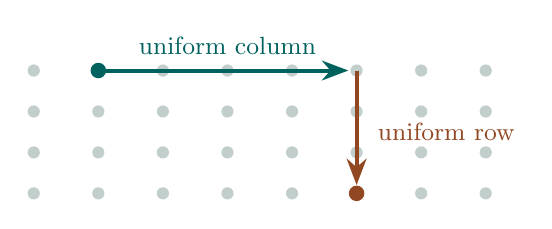
\begin{tikzpicture}[x=.82cm,y=.52cm,>=Stealth,font=\small]
  \foreach \x in {0,...,7} {\foreach \y in {0,...,3} {
    \fill[rulegray] (\x,\y) circle(2.2pt);}}
  \draw[teal,line width=1.45pt,->,shorten >=3pt] (1,3)--(5,3);
  \draw[copper,line width=1.45pt,->,shorten >=3pt] (5,3)--(5,0);
  \fill[teal] (1,3) circle(2.8pt);
  \fill[copper] (5,0) circle(2.8pt);
  \node[anchor=south,text=teal] at (3,3.16) {uniform column};
  \node[anchor=west,text=copper] at (5.18,1.5) {uniform row};
\end{tikzpicture}
\end{center}
Starting at \((u,v)\), choose a uniform column \(v'\) within row \(u\),
then a uniform row \(u'\) within column \(v'\). The endpoint \((u',v')\)
is uniform on the whole rectangle. Cyclic shifts suffice at each stage.
The Boolean circuit bound needs just \(t=1\). There is then one list, a single
uniform row move, and no column move. The rectangle restores the full batch
quantifier of the tensor theorem.

\subhead{Turn the wires into a regular graph}
Give each payload leg its own terminal vertex in the graph used for distances,
joined to its incident tensor by one edge. Pin the tags to permutations.
Assign input and output terminals to their designated sites, in all \(h\)
lanes. Four layers, two ends and \(h\) lanes give at most \(8h\) terminals
per site. Only the two designated moves enter the lower bound.
Distribute the remaining vertices evenly among the sites. This gives a
quotient multigraph \(G\) of maximum degree \(O(h+W/B)\), since the old
graph had maximum degree three. Pair the two ends of every edge as labels
and fill vacant labels by holding at the site. This gives a regular graph
of degree \(d=O(W/B)=O(hp)\). The total degree \(Bd=O(W)\).
A placement of the sites now specifies the position of every network vertex.

The same rectangle serves two purposes. The row and column moves give the
independent endpoints required by the obstruction. Grouping \(h\) payload
lanes at every position makes the number of demanded wires comparable to
the full batch, even if its original realization shares work between lists.

\newpage
\heading{From routing to a squared-distance bound}
For a placement \(f\) of the \(B\) sites, write \(P_q=\E_{i,j}d(f_i,f_j)^q\)
for independent uniform vertices and \(E_q=\E_{i\sim j}d(f_i,f_j)^q\)
for an oriented edge of the regular walk.

Pinning the tags realizes a product of equality wires on the prescribed
pairs, one in each lane. In a spectral space, the sum of their lengths
at their incident vertices is at most the sum of the internal wire lengths.
This is monotonicity under local tensor maps and additivity for independent
wires. The triangle inequality adds the two terminal edges per paired bit.
Average over the
row and column permutations. Summing the \(h\) lanes and using the triangle
inequality for the two moves gives
\[
             Bh P_1\le O(Bd) E_1,\qquad P_1\le K E_1,\quad K=O(p).
\]
This holds for every placement. It holds for real-valued functions with the
same constant as well. Put the two sides of a cut at two distinct points
of a spectral space and cancel the distance. Integrating over the threshold
cuts of a real function gives the scalar inequality. Across a cut, \(k\)
separated equality wires have rank \(2^k\), so at least \(k\) edges of the
augmented graph cross, counting terminal spokes. A one-point target has zero energy.
\matrixref{list.tex\#L60-L79}{OpenAI, wire-price inequality.}

\subhead{A first moment suffices}
Choose \(z\) with \(\E_i g_i\le K E_1\), where \(g_i=d(f_i,f_z)\).
Then \((\E g)^2\le K^2 E_2\). The scalar inequality applied to \(g^2\)
and \((a-b)^2\le|a^2-b^2|\) for \(a,b\ge0\) give
\[
 2\bigl(\E g^2-(\E g)^2\bigr)
 \le K\,\E_{i\sim j}|g_i^2-g_j^2|
 \le \E g^2+K^2 E_2 .
\]
For the last step use \(|g_i-g_j|\le d(f_i,f_j)\) and
\(K d(f_i,f_j)(g_i+g_j)\le (g_i^2+g_j^2)/2+K^2 d(f_i,f_j)^2\).
Regularity makes each endpoint uniform. Hence \(\E g^2\le3K^2 E_2\).
The triangle inequality through \(z\) now gives \(P_2\le12K^2 E_2\).

\subhead{Apply the logarithmic obstruction}
For a class without ports, a \(d\)-regular graph on \(B\ge2\) vertices
satisfying \(P_2\le\beta E_2\) for all placements in the class must have
\(\beta\ge c\log B/\log(d+1)\). This is the quantitative part of the
geometric argument. The integer form on page 6 bounds \(1+\beta\),
which gives the same routing estimate since \(p\ge3\).
\permref{entropy.tex\#L54-L64}{OpenAI, logarithmic Poincar\'e obstruction.}
Its proof explains the logarithm. A graph with too small a constant could
be inserted at every vertex of a preceding graph. Smoothing the old walk
before inserting the copies keeps the new constants bounded. Iteration would
produce bounded-degree graphs of unbounded order, hence ports.
Our graph has \(B\ge 2^h\) and \(d=O(hp)\), giving
\[
            p^2\log(2+hp)\ \gtrsim\ h,\qquad
            p\ \gtrsim\ \sqrt{h/\log h}.
\]
For the second inequality, separate \(p\ge h\) and \(p<h\). The estimate is
uniform over the entire batch range. The original uniform-destinations lemma
gives \(\sqrt h\). The rectangle loses a factor \(\sqrt{\log h}\) and retains
every fixed exponent below \(1/2\). It uses the independent-pair obstruction
directly. The source treats general destination distributions using entropy,
product closure and minimax. \matrixref{list.tex\#L45-L126}{OpenAI, original no-ports argument.}

\newpage
\heading{With ports, choose the batch before compiling}
Two results about arbitrary computation enter here. First, over a finite
field with ports, a normalized trivalent network with \(e\) exterior bits
and size at most \(m\), where \(M\le m\le M^4\), admits an exact compiler.
It produces \(d\) copies using trivalent gates and \(\Tag_h\) tests. Charging
all incidences, the size is \(S\le C d(m/h^a+e(1+\log h)^C)\) for some
\(a>0\). The factor satisfies \(1\le d\le D\) with
\(\log_2 D=O((\log h)^2)\), uniformly over these networks.
\geomref{exact.tex\#L11-L31}{OpenAI, Proposition 14.1.}

The compiler batches local contractions so their wiring descriptions can be
shared. Tagged permutation tests check the rearrangements of the resulting
records. This is where a cheap router would save work on arbitrary tensors.

Second, let \(U_\ell\) count signed computation paths of the source's
polynomially clocked universal machine on \(\ell\) input bits, in the
field. One copy has a polynomial-size verifier. For some \(\xi,\delta>0\),
all large \(\ell\) and all \(1\le j\le 2^{\ell^\xi}\), even a network
sharing work across \(j\) copies needs volume \(>j\ell^{1+\delta}\).
\permref{model.tex\#L21-L87}{OpenAI, construction and Theorem 12.1.}
The hard computation diagonalizes against a proposed cheap evaluator. A
program makes its signed count the evaluator's answer plus one, while exact
evaluation on its own description forces the two answers to coincide.
\permref{batch.tex\#L66-L89}{OpenAI, diagonal step.}

Write \(x(j)=\vol_F(U_\ell^{\otimes j})/(j\ell)\). Disjoint copies give a
polynomial upper bound, and on the hard interval \(x(j)>\ell^\delta\).
A minimum-volume realization can be normalized at cost at most three times
its volume. Subdivide each internal edge and give every exterior bit a separate
equality leaf. Each old labeling has one consistent extension. Compile this network. Replace the calls in
groups of \(t\) by the proposed network for \(\Tag_h^{\otimes t}\).
Every call exposes \(3Mh\) incidences. The last group is filled with
accepted constant inputs. Exact tensor equality makes substitution valid
even along wires joining two calls in one group. The new volume is
\(O(p(S+3tMh))\). For \(j\ge M^2\) and \(t\le2M\) this gives, when the
compiler size budget holds,
\[
 x(jd)\le C_1p\left(\frac{x(j)}{h^a}+(1+\log h)^{C_2}+\frac{6h}{\ell}\right). \tag{1}
\]

For a single proposed router (\(t=1\)), substitute it directly at every call.
There is no incomplete group, so the last term in (1) drops out.

\subhead{One finite choice of scale}
If \(x\ge1\) on \([j_0,j_0D^L]\) and \(x(j_0)<2^L\), there is a \(j\)
with \(j_0\le j\), \(jD\le j_0D^L\), \(x(j)\le x(j_0)\) and
\(x(jd)\ge x(j)/2\) for \emph{every} \(1\le d\le D\).
Take any multiplier that more than halves the cost while one exists.
After \(L\) moves the cost would be below one. At the first stopping point
there is room for one more multiplier. This choice uses the profile alone.

Take an integer \(b>\max(2,1/\xi,a/\delta)\), \(\ell=h^b\) and \(j_0=M^2\).
Choose \(A\) with \(x(j_0)\le h^A\) and \(L=\lfloor A\log_2 h\rfloor+1\).
Then \(j_0D^L\le M^3\), since \(L\log_2D=O((\log h)^3)=o(h)\).
The chosen network admits a normalized size budget in \([M,M^4]\), since
its volume is at most \(M^3\ell h^A\) before normalization.
Also \(3h\le\ell^\xi\), so the whole window lies in the hard interval.
As \(b\delta>a\), the two additive terms in (1) total at most \(x(j)/h^a\)
eventually. The one use of the compiler must therefore satisfy
\[
             \tfrac12 x(j)\le x(jd)\le 2C_1p\,x(j)/h^a,
                  \qquad p\ge h^a/(4C_1).
\]

\subhead{Why the hard computation needs a batch theorem}
Over \(\mathbb F_2\), counting trivalent networks gives a table of \(T=2^{2h}\)
bits whose one-query volume is \(\Omega(T/h)\). For \(d\) queries, sort one
hardwired dictionary together with all queries and scan each key's answers.
The product of all answers costs \(O((T+d)h\log^2(T+d))\) binary gates.
The compiler's construction has \(h^{9/2}\le d=h^{O(1)}\) and \(a<0.02\).
At this scale the dictionary costs \(o(dT/h^{1+a})\). Ordinary counting
therefore cannot provide the needed lower bound on the replicated workload.
\geomref{exact.tex\#L98-L185}{OpenAI, choice of replication parameters.}

\newpage
\heading{From one list to all Boolean circuits}
In either field case \(W/(tMh)\) grows as a positive power of \(h\), uniformly
for \(1\le t\le2M\). Put \(w=h+1\), so \(n_w=2w\,2^w=4M(h+1)\).
Unary contraction on page 1 gives the finite-field list-volume theorem for
some \(\varepsilon>0\) depending only on the fixed field. Decreasing the
exponent absorbs the constants, yielding
\[
               \vol_F(\ED_w^{\otimes t})>t n_w w^\varepsilon
       \quad\bigl(w\text{ sufficiently large},\ 1\le t\le2^w\bigr).
\]
This gives precisely the batch range in
\matrixref{obstruction.tex\#L46-L60}{OpenAI, Theorem 2.2.}

Fix \(F=\mathbb F_2\). Let a single-output Boolean circuit on \(N\) input
bits have \(s\) gates. The basis contains every binary truth table and both
nullary constants. Unary operations can ignore one input. Only gates count
toward \(s\). Represent each gate by its table. Equality vertices distribute
a signal to its consumers and the output is pinned to one. Every accepted
input has exactly one consistent internal trace. The native circuit compiler
gives trivalent volume at most \(2N+8s+5\). Depth and fan-out are unrestricted.

For \(m\) records of width \(2\lceil\log_2 m\rceil\), take
\(w=\lceil\log_2m\rceil-1\). Then \(2^w<m\le 2^{w+1}\). Embed a short
list of \(2^w\) records of \(2w\) bits in the circuit input. Append two zero
bits to each short record. Fill the other rows with distinct fixed records
ending in two one bits. There are at most \(2^w\) such extra rows.
Distinctness of the large list is precisely distinctness of the short list.
Each short input bit occurs once, so the same pinning operation gives a
network for \(\ED_w\), even when \(m\) is a power of two.

For \(w\ge2\), \(N=2m(w+1)\le4n_w\) and \(\log_2 N\le4w\).
Consequently \(2N+8s+5\ge\vol_F(\ED_w)>n_w w^\varepsilon\).
For all sufficiently large \(m\) this implies
\[
           s>c\,N(\log_2 N)^\varepsilon,\qquad
           c=1/(64\cdot4^\varepsilon).
\]
Taking the minimum over circuits and letting \(m\) grow gives a size greater
than \(AN\) eventually for every fixed real \(A\). The circuit compiler works
over any field. Thus a single field without ports would already give
\(N(\log_2 N)^\varepsilon/128\) for each fixed \(0<\varepsilon<1/2\).
The dichotomy avoids needing to decide which case holds for \(\mathbb F_2\).

\subhead{Provenance and formal status}
The target theorem, field split and companion theorems come from OpenAI's
24 November 2026 preprints. This derivation changes the signed projection,
the rectangle argument, and the choice of workload scale.

The verification problems also reduce in reverse. Guess destination ranks
and a strictly increasing table of full records. A distinct list has exactly
one accepting witness, its sorted order. For \(2w\)-bit records, split each
payload into two \(w\)-bit lanes. Use address \((\mathrm{rank}_i,\mathrm{lane})\)
in one \(\Tag_{w+1}\) on \(2^{w+1}\) positions and pad each lane with one
zero. Copying ranks and checking adjacent ordered records costs
\(O(2^w w)\) trivalent volume. Lean checks the sorted-witness identity.
The converse volume estimate above is a paper argument.

Lean checks the signed projection on joint networks, the direct circuit
construction and the all-length transfer. It proves the field-without-ports
bound using actual finite wire exponents. The ports branch still uses the
two companion results on page 4 as mathematical inputs. The Lean transfer
assumes their exact compiler and hard signed verifier in the ports case. It
constructs the minimizing networks, checks substitution and the choice of
scale, and derives both the batch bound and the eventual gate bound.
\href{https://github.com/cslib-community/cslib-frontier/issues/8448}{cslib-frontier issue 8448.}

\newpage
\heading{Why one good graph would create ports}
Let \(H\) have \(n\ge2\) vertices, degree \(d\ge1\), and a common bound
\(P_2\le b E_2\) for all placements into a family of complete CAT(0) spaces.
Starting from one vertex with loops, we will construct graphs with \(n^k\)
vertices, degree \(2d\) and a single common bound. The construction works if
\(n\ge(8d)^{2s}\) for an integer \(s\ge7000(1+b)\). The walk smoothing and
amplification come from \permref{entropy.tex\#L4-L117}{OpenAI, Lemma 4.1 and
Theorem 4.2.}

\subhead{Smooth the old graph}
Let \(P\) be the old walk, \(A=(I+P)/2\), and \(\pi\) its stationary law.
For two placements \(x,z\), write \(J(K;x,z)=\mathbb E d(x_i,z_j)^2\)
where \(i\sim\pi\) and \(j\sim K(i,\cdot)\). Replace each \(z_i\) by the
barycenter \((B_Az)_i\) of its one-step neighbors. The CAT(0) variance
inequality and stationarity give
\[
  J(KA;x,z)\ \ge\ J(K;x,B_Az)+J(A;B_Az,z)
\]
for stationary \(K\). Iteration sums the energy lost at successive steps.
Averaging the first \(2s\) inequalities yields a placement \(y\) for which
\[
 J(I;x,y)+2sJ(P;y,y)\ \le\
         16\cdot\frac1{2s}\sum_{j=1}^{2s}J(A^j;x,x).
\]
Passing through \(y\) moves both endpoints of a pair. An old all-pairs
bound \(\gamma\) consequently becomes \(48\max(2,\gamma/(2s))\) for
the average walk on the right.

\subhead{Fit the labels, then replace each vertex}
To realize the average exactly, choose a walk length uniformly from \(1\)
through \(2s\), then read that many letters of a uniformly chosen length-\(2s\)
word. At degree \(2d\) the lazy alphabet has \(4d\) letters. The number
of labels is \(2s(4d)^{2s}\le(8d)^{2s}\). Pack complete copies of this
alphabet into \(n\) labels, filling the remainder with holding steps. At
least half the resulting transition law still samples the average.

Replace every old vertex by a copy of \(H\) on its \(n\) labels. Half of
the new walk stays within that fiber, half follows the old matching.
In each fiber choose an actual vertex whose average squared distance
to the others is at most the fiber's all-pairs average. Route a pair
through these two representatives and apply the triangle inequality.
If the fitted outer walk has bound \(a\), the new bound is at most
\(36(1+a)(1+b)\). This step works in every pseudometric space.

Take \(\gamma=6948(1+b)\). The fitted outer bound is at most \(192\), and
\(36(1+192)(1+b)=\gamma\). Each iteration multiplies the order by \(n\)
and restores the same constant. A family without ports therefore satisfies
\[
                  n<(8d)^{2\lceil7000(1+b)\rceil}.
\]
Lean tests all multiplicative upper functionals. A squared-energy bound passes
to limits and common rescalings, and every finite price is the pullback of a
complete CAT(0) price metric. This gives the native finite test. The paper's
normalized additive points satisfy the upper-functional axioms: a sum of local
restrictions is a restriction of their direct sum. Hence native ports imply the
paper's ports, the direction used by the compiler.
\href{https://github.com/cslib-community/cslib-frontier/blob/c258d64a931afcaaf6259abeec215b32e72360e2/CslibFrontier/Computability/Circuit/Arithmetic/Separation/Curvature/Curvature.lean}{Native price realization.}
\geomref{prices.tex}{OpenAI, spectral points}
and \geomref{port-graphs.tex\#L10-L36}{Definition 11.1.}
\end{document}
